% !TeX root = RJwrapper.tex
\title{Techniques for Evaluating Clustering Data in R. The \pkg{Clustering} Package}
\author{by Luis Alfonso Pérez, Ángel Miguel García Vico, Pedro González and Cristóbal J. Carmona}

\maketitle

\abstract{
Clustering is an unsupervised learning technique where the model is adjusted to the observations. This technique is quite common among researchers because they can obtain knowledge quickly and easily. The use of this technique is suitable for automatically classifying data to reveal concentrations of data. This paper presents the \pkg{Clustering} package which contains a sest of clustering algorithms with two objectives: first grouping data in an homogeneous way by establishing differences between clusters, and second generating a ranking between algorithms and the variables analysed in the dataset. This package contains references to other R packages without using external software. As a complement to the standard execution through the console, it incorporates a GUI through which we can execute the package without having to know the parameters.

}

\section*{Introduction}

Exploring the properties of information in order to make groups is an unsupervised learning technique known as clustering \citep{b46} \citep{b47}. This technique is a concise data model where a set of data must be partitioned and introduced in groups or clusters. These clusters must meet two conditions: clusters must be the most disparate possible among them, and the elements that contain them the most similar. If we review the literature related to clustering we can see that the fields where they can be applied are multiple, among which we highlight the following: Identify tourists and analyze their destination patterns from location-based social media data \citep{b1}, clustering algorithm that maximizes performance on 5G heterogeneous networks \citep{b2}, Application of data mining techniques to agriculture data \citep{b3}, Weighting of characteristics based on strength between categories and within categories for the analysis of feelings \citep{b4}, Music classification, genres and taste patterns \citep{b5}, Predict the direction, maximum, minimum and closing prices of the daily exchange rate of bitcoins \citep{b6} and Clustering of people in a social network based on textual similarity \citep{b7}.\\
As a rule, the clustering algorithms are based on the optimization of an objective function, which is usually the weighted sum of the distance to the centers, although these functions may vary and in some cases consists of the definition of functions. In the literature we can group the data in different ways among which we highlight \citep{b48}: partitional, hierarchical or based on density. One of the best known algorithms that solves the clustering problem is the k-means \citep{b49}\\
Throughout the literature we have located a wide variety of frameworks that work with clustering algorithm implementations among which we can cite the following: Weka \citep{b13}, ClustVis \citep{b14} and Keel \citep{b15} among others. Also within R there is a specific Cluster task view. Inside this section we see two well differentiated parts: on one hand we have the most outstanding packages by functionality and in second place we observe the set of packages that work with cluster ordered. From the set of packages we highlight the following: \pkg{ClusterR} \citep{b9}, \pkg{apcluster} \citep{b10}, \pkg{cluster} \citep{b11}, \pkg{advclust} \citep{b12} as well as alternatives to the traditional implementation of k-means and agglomerative hierarchical clustering.\\
This contribution presents the \pkg{Clustering} package. It is a package that allows you to compare multiple clustering algorithms simultaneously and assess the accuracy of the results. The purpose of this package is to evaluate a set of datasets to determine which variables are most suitable for clustering. So we can make evaluations of the clusters created, how they have been distributed, if the distributions are uniform or how they have been categorized from the data.\\
The distribution of the content of this contribution is as follows: Firstly, in section \ref{clusteringsec} we have the  presentation of clustering, types of clustering and similarity measures. Section \ref{internalandexternalmetricssec} presents the definition of the evaluation measures in order to value the distribution of the data in the clusters and finally Section \ref{clusteringpackage} describes the structure of the package and it presents a complete example about the use of the package.

\section*{Clustering}\label{clusteringsec}

Cluster analysis is an unsupervised learning method that constitutes a cornerstone of an intelligent data analysis process. It is used for the exploration of inter-relationships among a collection of patterns, by organizing them into homogeneous clusters. It is called unsupervised learning because unlike classification (known as supervised learning), no a priori labeling of some patterns is available to use in categorizing others and inferring the cluster structure of the whole data \citep{b17}. The basic concept of clustering should be expressed as follows:
\\
\begin{quote}
Clustering is the process of identifying natural clusters or clusters within multidimensional data based on some measure of similarity (Euclidean, Manhattan) \citep{b18}.
\end{quote}


This is a base definition of the clustering so variations in the problem definition can be significant, depending mostly on the model specified. For example, a generative model should define similarity based on a probabilistic generative mechanism, while a distance-based approach will use a traditional distance function to quantify it. In addition, the types of data specified also have a significant impact on the problem definition.

\subsection*{Clustering types}

There are a variety of clustering algorithms that can be classified into: hierarchical, partitioning, density-based, grid-based and probability distribution. The most commonly used groupings are: hierarchical, part-based and density-based.
\\
\begin{itemize}
  \item Hierarchical clustering algorithms: create a hierarchical breakdown of data into a dendogram that recursively divides the data set into smaller and smaller data. It can be created in two ways: bottom-up or top-down \citep{b19}. In bottom-up trees also known as agglomerative, as the objects are successively combined according to the measurements, until they are all joined into one or meet a completion condition.  In the case of top-down, it is known as divisive, where all the objects are in the same group, and as we iterate they are divided into smaller subsets, until each object is in an individual group or fulfills a condition of completion. An example of this type of clustering can be found in the Figure ~\ref{fig:hierarchical}. Some hierarchical grouping algorithms that belong to this sorting mode are CURE \citep{b20}, CHAMELEON \citep{b21}, and BIRCH \citep{b22}.
\begin{figure}[htbp]
  \centering
   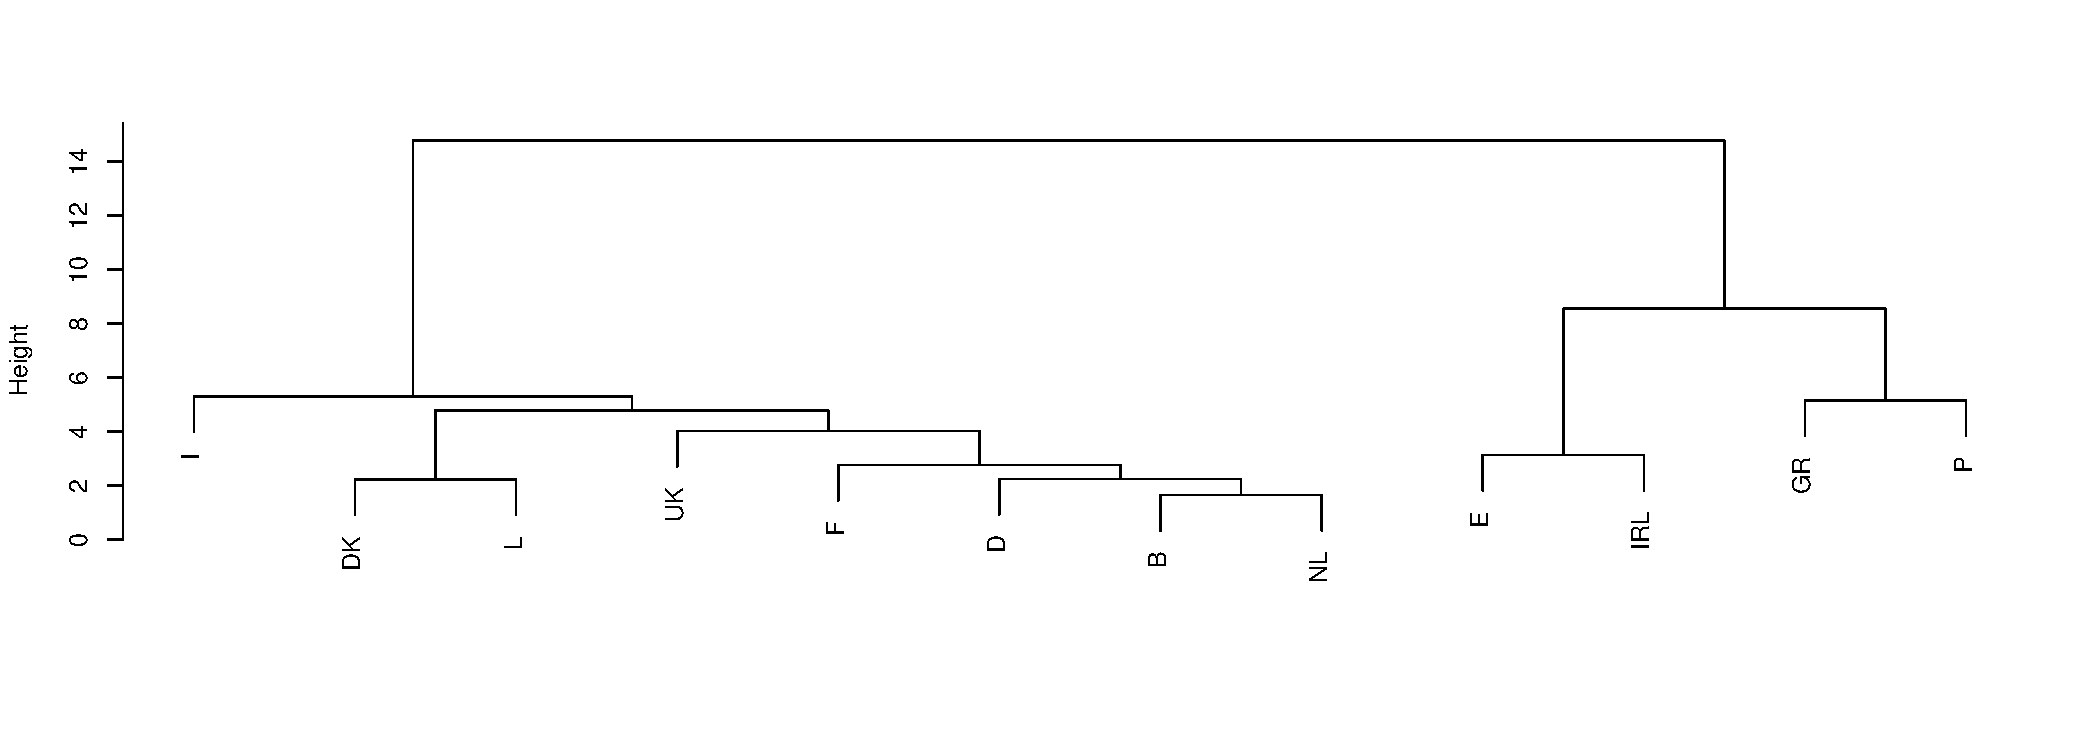
\includegraphics[width=14cm, height=4.5cm]{img/hierarchical.pdf}
    \caption{Hierarchical Clustering}
    \label{fig:hierarchical}%
\end{figure}
  \item Partial clustering: is considered to be the most popular of the clustering algorithms \citep{b23}. Such an algorithm is also known as an iterative relocation algorithm. This algorithm minimizes a given clustering criterion by iteratively relocating data points between clusters until an optimal partition is reached. This type of algorithm divides the data points into a partition
k, where each partition represents a cluster.
Partial clustering organizes the objects within k clusters so that the total deviation of each object from the center of its cluster or from a cluster distribution is minimal. The deviation of a point can be evaluated differently according to the algorithm, and is generally known as a similarity function.
If we want to observe graphically how this type of clustering works we can see it in the Figure ~\ref{fig:partitional}. Among the partitioning clustering algorithms we can find CLARANS, CLARA \citep{b24}, K-prototype \citep{b25}, K-mode \citep{b26} and K-means \citep{b27}.
\begin{figure}[htbp]
  \centering
   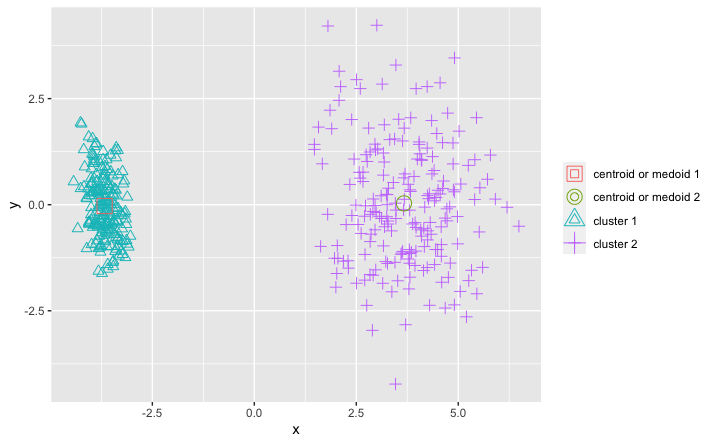
\includegraphics[width=14cm, height=4.5cm]{img/partitional}
    \caption{Partitional Clustering}
    \label{fig:partitional}%
\end{figure}
\\
  \item Density-based algorithms: obtain clusters based on dense regions of objects in the data space that are separated by low-density regions (these isolated elements represent noise). These regions are represented in the Figure ~\ref{fig:density}. Among the density-based algorithms, we highlight the following: Dbscan \citep{b28}, and Denclue \citep{b29}.
  \begin{figure}[htbp]
  \centering
   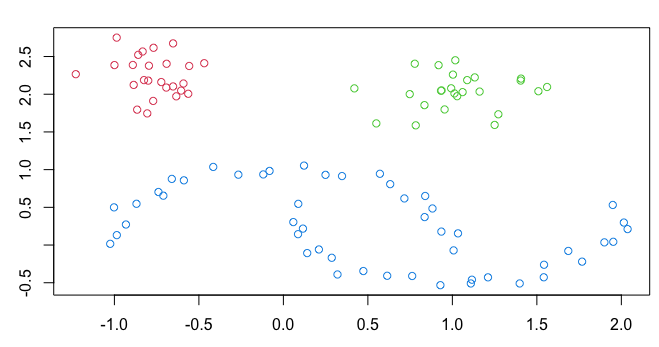
\includegraphics[width=14cm, height=5cm]{img/density}
    \caption{Density Clustering}
    \label{fig:density}%
\end{figure}
  \item Grid-based clustering algorithms: first quantize the clustering space into a finite number of cells and then perform the required operations on the quantized space \citep{b30}. Cells that contain more than certain number of points are treated as dense and the dense cells are connected to form the clusters. Some of the grid-based clustering algorithms are: STING \citep{b31}, Wave Cluster \citep{b32} and CLIQUE \citep{b33}.
  \item Model-based methods: are primarily based on a probability distribution. To be able to measure similarity it is based on the mean values and the algorithm tries to minimize the square error function. Auto Class algorithm uses the Bayesian approach, starting with a random initialization of parameters that is gradually adjusted in order to find the maximum probability estimates. AAmong the model-based algorithms we highlight SOM \citep{b34}. Model-based clustering is shown in the Figure ~\ref{fig:model}.
    \begin{figure}[htbp]
  \centering
   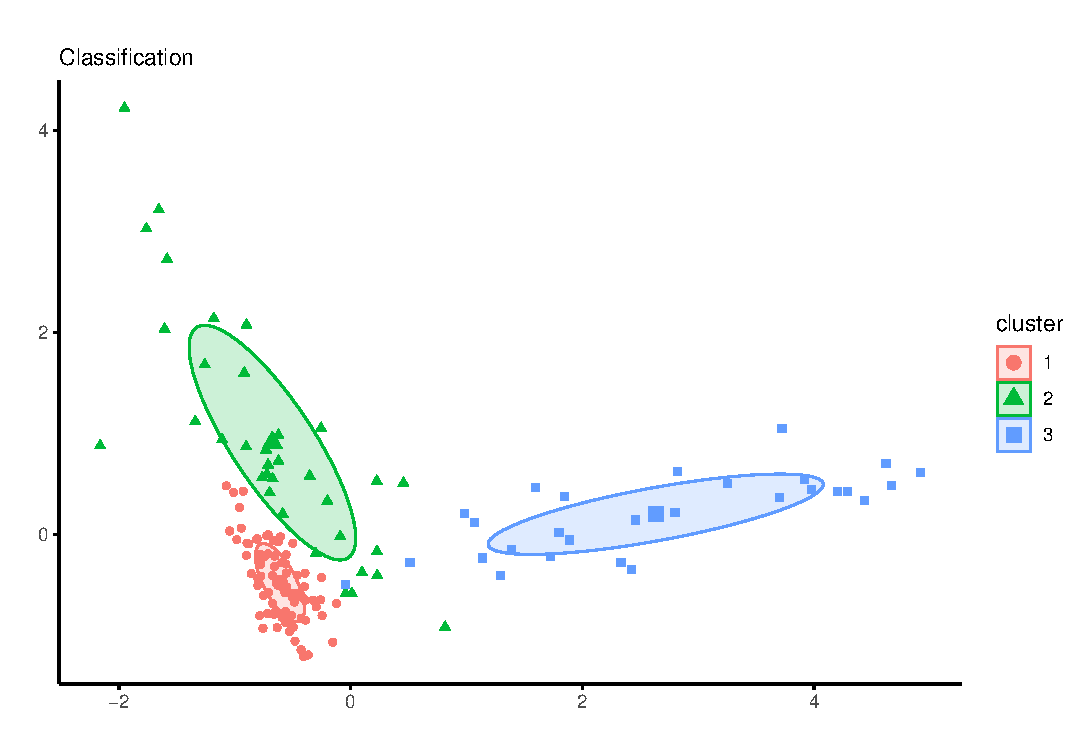
\includegraphics[width=14cm, height=4.5cm]{img/model}
    \caption{Model-Based Clustering}
    \label{fig:model}%
\end{figure}
\end{itemize}

\subsection*{Dissimilarity measures}

Dissimilarity measurements are important because they allow us the creation of clusters with the closest neighbours and the detection of anomalies, and they are also used in a large number of data mining techniques. It is also a measure that determines the degree to which objects are different. We often use the term distance as a synonym for dissimilarity. The values of dissimilarity should be in the range [0,1], but it is common to find in some cases the range 0 to $\infty$.
\\
Many distance measures have been proposed in literature for data clustering. The choosing an appropriate similarity measure is also crucial for cluster analysis, especially for a particular type of clustering algorithms. For example, the densit -based clustering algorithms, such as DBScan \citep{b28}, rely heavily on the similarity computation. Density-based clustering finds clusters as dense areas in the data set, and the density of a given point is in turn estimated as the closeness of the corresponding data object to its neighboring objects \citep{b50} \citep{b51}.
\\
As measures of dissimilarity in clustering we highlight the following:

\begin{itemize}
  \item Minkowski: Is a metric in a normed vector space which can be considered as a generalization of both the Euclidean distance and the Manhattan distance \citep{b56}.
    \begin{equation}
        d_{min} = (\sum_{i=1}^{n}|x_i - y_i|^m)^\frac{1}{m}, m\geq 1
    \end{equation}
    where m is a positive real number and xi and yi are two vectors in n-dimensional space.
    \item Euclidan distance: Is a special case of Minkowski distance. Is a measure of the true straight line distance between two points in Euclidean space. \citep{b57}.
    \begin{equation}
        d_{xy} =  \sqrt{\sum_{i=1}^{n}(X_{i}-Y_{i})^2}
    \end{equation}
     \item Manhattan distance: Also known as the geometry cab driver is defined as the
sum of the lengths of the projections of the line segment between the points onto the coordinate axes \citep{b58}.
     \begin{equation}
        d_{xy} =  \sum_{i=1}^{n}|X_{i}-Y_{i}|
    \end{equation}
    \item Mahalanobis distance: Is a data-driven measure in contrast to Euclidean and Manhattan distances that are independent. It is in charge of measuring the distance in a multivariate space \citep{b58}.
    \begin{equation}
        d_{mah}= \sqrt{(x-y)S^-1(x-y)^T}
    \end{equation}
    where S is the covariance matrix of the dataset
    \item Pearson correlation: It’s a statistically based metric that measures linear correlation between two variables x and y.
    \begin{equation}
        Pearson(x,y)= \frac{\sum_{i=1}^n(x_i-\mu_x)(y_i-\mu_y)}{\sqrt{\sum_{i=1}^n(x_i-y_i)^2}\sqrt{\sum_{i=1}^n(x_i-y_i)^2}}
    \end{equation}
    where $\mu_x$ and $\mu_y$ are the means for x and y respectively.
    \item Jaccard Index: Is a classical similarity measure on sets with a lot of practical applications in information retrieval, data mining, machine learning, and many more \citep{b35} \citep{b59}. It measures the similarity of the two data elements as the intersection divided by the union of the data elements as shown below:
    \begin{equation}
        J(A,B) = \frac{A \cap B}{A \cup B}
    \end{equation}
    \item Gower distance: It is a measure of similarity that allows the simultaneous use of quantitative, qualitative and dichotomous variables. By applying this similarity coefficient can be to determine the degree of similarity between individuals; who have been measured qualitative, quantitative characteristics (continuous and discrete) and binary.
    \begin{equation}
        d_{ij}=\sqrt{(1-S_{ij})}
    \end{equation}
    where $S_{ij}$ is Gower similarity coefficient.
\end{itemize}

\section*{Internal and External clustering validation measures}\label{internalandexternalmetricssec}

Clustering validation is a technique to find a set of clusters that best fits natural partitions (number of clusters) without any class information.The results of a clustering algorithm are known as cluster validity. The following criteria must therefore be taken into account when investigating the validity of clusters. The first criterion is based on external measures, which involves evaluating the results of a base algorithm in a pre-specified structure which is imposed on a data set and reflects our intuition about the structure of clustering of the data set. The second criterion is based on internal measures where it evaluates the results of a clustering algorithm in terms of the quantity involved in the vectors of the dataset itself (e.g. the proximity matrix). And as a third criterion known as relative criterion whose purpose is to compare the results of execution of an algorithm with another using different parameters.
When we talk about criteria based on internal measures we must take into account the criteria of compaction and separation \citep{b53} \citep{b52} as you can see in the Figure ~\ref{fig:cohesion}:
\begin{enumerate}
  \item Compactness, the members of each cluster should be as close to each other as possible. A common measure of compactness is the variance, which should be minimized.
  \item Separation, the clusters themselves should be widely spaced. There are three common approaches measuring the distance between two different clusters:
  \begin{itemize}
  \item Single linkage: It measures the distance between the closest members of the clusters.
  \item Complete linkage: It measures the distance between the most distant members.
  \item Comparison of centroids: It measures the distance between the centers of the clusters.
\end{itemize}
\end{enumerate}
These criteria are graphically represented in the image ~\ref{fig:separation}

\begin{figure}[htbp]
  \centering
    \subfloat{{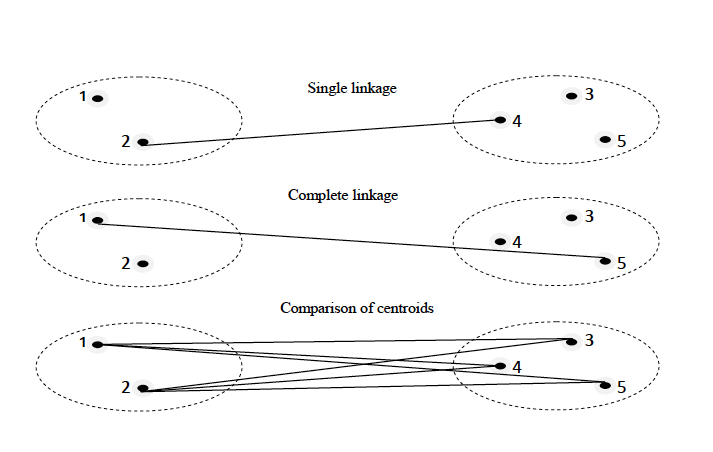
\includegraphics[width=14cm,height=6cm]{img/separation} }}%
    \caption{Intercluster distance \citep{b60}}%.
    \label{fig:separation}%
\end{figure}

Inside external tests exits some measures to evalute clustering results. Among which we highlight:

\begin{itemize}
    \item Entropy:It evaluates the distribution of categories in a cluster \citep{b40}.
    \begin{equation}
        Entropy =  \sum_{j=1}^{m} \frac{n_{j}}{n}E_{j}
    \end{equation}
    Where $n_{j}$ is the cluster size j, n is the number of clusters, and m is the total number of data points. To calculate the entropy of a data set, we need to calculate the class distribution of the objects in each group as follows:
    \begin{equation}
        E_{j} =  \sum_{i} p_{ij}log(p_{ij})
    \end{equation}
    Where $p_{ij}$ is the probability of a point in the cluster $i$ of being classified as class $j$.
    \item Recall: It indicates the proximity of the measurement results to the true value \citep{b41}.
    \begin{equation}
         Recall(i,j) = \frac{n_{ij}}{n_{i}}
    \end{equation}
    $n_{ij}$ is the number of objects of class i that are in cluster j, $n_{j}$ is the number of objects in cluster j and $n_{i}$ is the number of objects in cluster i.
    \item Precision: It refers to the dispersion of the set of values obtained from repeated measurements of one magnitude \citep{b41}.
        \begin{equation}
            Precision(i,j) = \frac{n_{ij}}{n_{j}}
        \end{equation}
     $n_{ij}$ is the number of objects in class i that are in cluster j, $n_{j}$ is the number of objects in cluster j and $n_{i}$ is the number of objects in class i.
    \item F-measure: It merges the concepts of accuracy and recall of the retrieved information \citep{b42}. Therefore, we calculate the cluster accuracy and recall for each class as:
    \begin{equation}
        F-measure(i,j) = \frac{2 * (Precision(i,j) * Recall(i,j))}{(Precision(i,j) + Recall(i,j))}
    \end{equation}
    \item Fowlkes-Mallows Index: It is a measure of comparison of hierarchical clustering, however it can also be used in flat clustering since it consists of the calculation of an index $B_{i}$ for each level i = 2 ,..., n-1 of the hierarchy \citep{b43}. The measure $B_{i}$ is easily generalizable to a measure for clustering of different clusters. It can therefore be said that Fowlkes is a measure that can be interpreted as the geometric mean of accuracy (ratio between the number of relevant documents recovered and the total number of documents recovered).
    \begin{equation}
        Fowlkes = \sqrt{\frac{TP}{TP + FP}*\frac{TP}{TP + FN}}
    \end{equation}
    \begin{equation}
        Fowlkes = \sqrt{Precision*Recall}
    \end{equation}


    \item Variation information: Variation in information or distance of shared information is a measure of distance between two groups \citep{b43}. This measure is closely related to mutual information (mutual dependence between the two variables). However, in contrast to mutual information, variation of information is a true metric, in the sense that it is due to the inequality of triangles (for any triangle, the sum of the lengths of any two sides must be greater than or equal to the length of the remaining side).
    \begin{equation}
       VI = - \sum_{i}^{j} r_{ij}\left[\log\left(\frac{r_{ij}}{p_{i}}\right) +\left(\frac{r_{ij}}{q_{j}} \right)\right]
    \end{equation}
\end{itemize}

As with the external measures, we will now list the most relevant internal measures:
\begin{itemize}
    \item Connectivity: This measure reflects the extent to which items placed in the same group are considered their closest neighbours in the data space, i.e. the degree of connection of the clusters should be minimal \citep{b39}.
    \begin{equation}
        connectivity = min_{ 1\leq i \leq K} \left( min_{1\leq j \leq K, i\not= j} \left( \frac{dist(C_i,C_j)}{max_{1\leq k \leq K} \lbrace diam(C_k) \rbrace }  \right) \right)
    \end{equation}
    Where $dist(C_i,C_j)$ is the distance between two clusters and $diam(C_k)$ is diameter of a particular cluster.
    \item Dunn: It represents the relationship of the smallest distance between observations that are not in the same cluster and the largest distance within the same cluster \citep{b44}.
    \begin{equation}
    dunn =  min_{1_\leq i\leq k} \left( min_{i+1\leq j \leq k}  \left( \frac{dist(C_i,C_j)}{max_{1_\leq l \leq k} diam(C_{l})} \right) \right)
    \end{equation}
    Where $dist(C_{i},C_{j})$ is distance between clusters $C_{i}$ and $C_{j}$ and $diam(C_{l})$ is diameter of cluster $C_{l}$.
    \item Silhouette index: The silhouette value is a measure of how similar an object is to its own cluster (cohesion) compared to other clusters (separation) \citep{b45}.
    \begin{equation}
        S = \frac{1}{N}\sum_{i=0}^{N}\frac{b_{i} - a_{i}}{max(a_{i},b_{i})}
    \end{equation}
    where $$a_{i}=\frac{1}{|C_{j}| - 1} \sum_{y\in C_{j},y\neq x_{i}}^{}\|y-x_{i}\|$$ and
    $$ b_{i} = \min\limits_{l \in H, l\neq j}^{} \frac{1}{|C_{l}|} \sum_{y \in C_{l}}^{} \| y - x_{i} \| $$ with
    $$ x_{i} \in C_{j}, H = \{h: 1 \leq h \leq K\}$$
\end{itemize}

The above evaluation measures can be grouped into families in order to evaluate the quality of the clusters. If we look at the Figure~\ref{fig:external} we can group Entropy, Recall, Precision, F-Measure, Fowlkes-Mallows Index and Variation information into three families \citep{b54}:

\begin{figure}[htbp]
  \centering
    \subfloat{{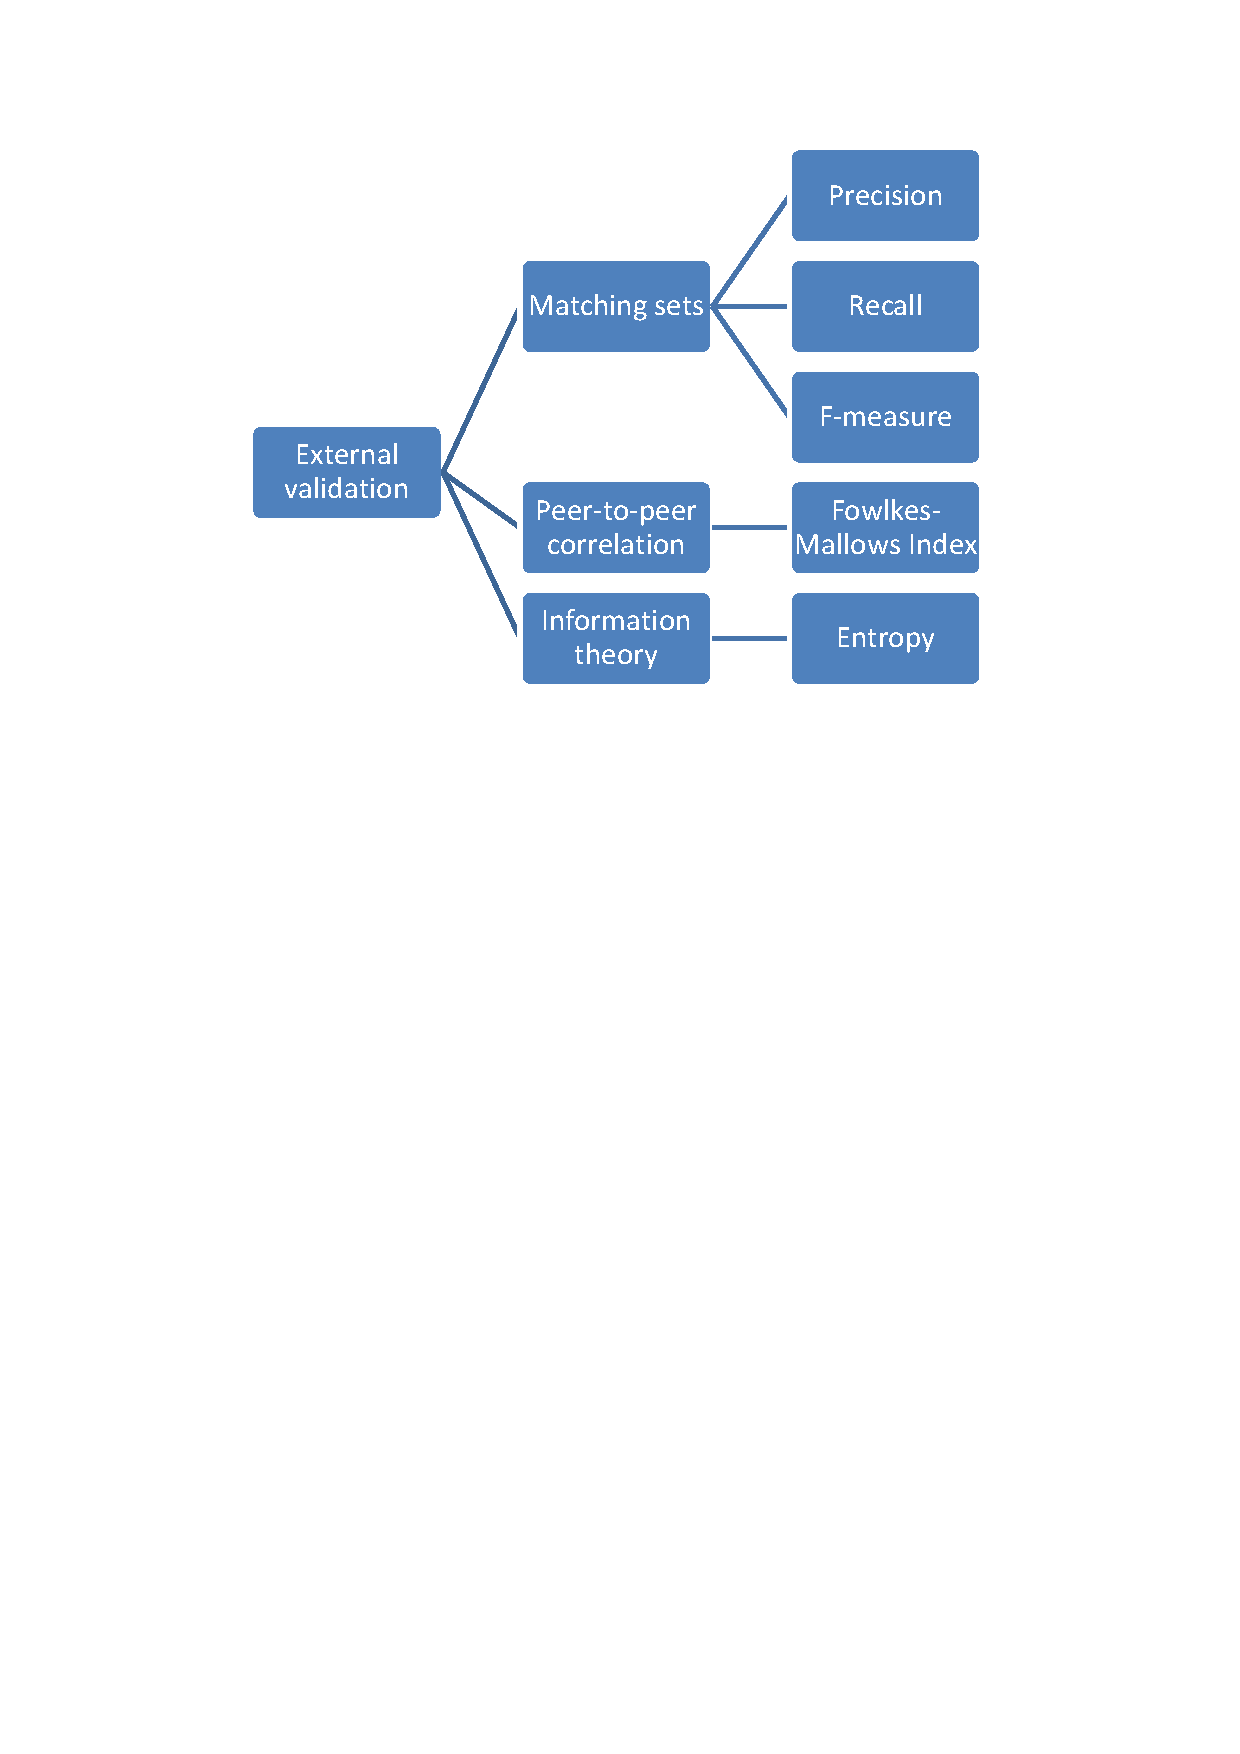
\includegraphics[width=6.5cm,height=6cm]{img/external} }}%
    \caption{External validation methods \citep{b54}.}%
    \label{fig:external}%
\end{figure}

\begin{itemize}
  \item Matching Sets: used to compare two partitions of data consists of those method that identify the relationship between each cluster detected in C and its natural correspondence to the classes in the reference result defined by P (clustering result prediction) \citep{b54}.\\
Several measures can be defined to measure the similarity between the clusters in C, obtained by the clustering algorithm, and the clusters in P, corresponding to our prior (external) knowledge. The metrics included in this method are: Precision, Recall and F-measure.
  \item Peer-to-peer Correlation: are based on the correlation between pairs, i.e., they seek to measure the similarity between two partitions under equal conditions, such as the result of a grouping process for the same set, but by means of two different methods C and P \citep{b54}. It is assumed that the examples that are in the same cluster in C should be in the same class in P, and viceversa. We highlight the following metrics: Fowlkes-Mallows Index.
  \item Measures Based on Information Theory: A third family is based on Information Theory concepts, such as the existing uncertainty in the prediction of the natural classes provided by the partition P \citep{b54}. This family includes basic measures such as entropy and variation information.
\end{itemize}

Internal evaluation metrics (see Figure ~\ref{fig:cohesion}) do not require external information, so they are focused on measuring cohesion (how close the elements are to each other) and separation (they quantify the level of separation between clusters).

\begin{figure}[htbp]
  \centering
    \subfloat{{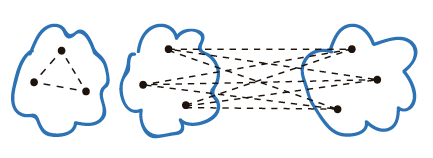
\includegraphics[width=8.5cm, height=4cm]{img/cohesion} }}%
    \caption{Representation of cohesion and separation in clustering \citep{b54}.}%
    \label{fig:cohesion}%
\end{figure}

According to the figure ~\ref{fig:internal}, the internal Dunn, Silhouette and Connectivity metrics are based on the concepts mentioned above so we can group them as partitioning methods.

\begin{figure}[htbp]
  \centering
    \subfloat{{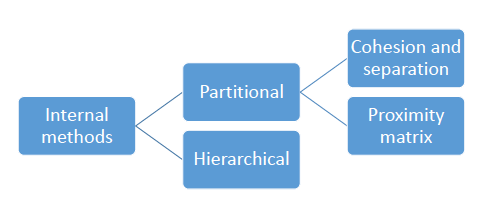
\includegraphics[width=6.5cm]{img/internal} }}%
    \caption{Internal validation methods \citep{b54}.}%
    \label{fig:internal}%
\end{figure}

\section{The \pkg{Clustering} package}\label{clusteringpackage}
\pkg{Clustering} package is a package that has been written entirely in R language. The package contains other \pkg{Clustering} packages that run hierarchical, partitional and agglomerative hierarchical algorithms. As an addition to the package it has been provided with the ability to read data in different formats such as CSV, KEEL, ARFF (Weka) and \texttt{data.frame} objects. Most of the methods have been provided with a set of default parameters, so we can easily run our algorithm without knowing the parameters. Reviewing the related implementations on Clustering, until now the algorithms were run in parallel. In the case of needing to execute many algorithms simultaneously we cannot do it, since we must do it individually. Moreover, if an algorithm has implemented several measures of dissimilarity, it is necessary to perform as many executions as measures have, so it requires a lot of time and in some cases can lead to confusion in the executions. Besides, when we evaluate the clustering results it is necessary to indicate a variable of the data set, so the execution times increase more and not only that, but also depending on the chosen variable it can vary in the results so with this package we will try to solve this problem. With the Clustering package we will be able to execute simultaneously several algorithms for each of the implemented similarity measures. In addition, when evaluating the results of the executions, we have a set of measures that are executed together, which until now was done one execution per measure. It is possible to incorporate new measures quickly in the future. Another problem we are solving is whether the choice of one or another dataset variable influences the quality of the results. Therefore, this problem is solved by carrying out executions for each of the variables. The package shows the results visually, so we can draw conclusions more quickly.  Thanks to this package we solve many of the problems encountered.

\subsection{Algorithms of the package}
These are the algorithms available within the package, which we will classify as follows:
\begin{itemize}
  \item Hierarchical Clustering: \texttt{agnes, clara, daisy, diana, fanny, fuzzy\_cm, fuzzy\_gk, fuzzy\_gg, hcluster, mona, pam, pvpick and pvclust.}
  \item Partitioning Clustering: \texttt{gama, gmm, kmeans}
  \item Aglomerative Clustering: \texttt{aggExCluster, apclusterK}
\end{itemize}

\subsection{Package Architecture}

The main class of the package is the \pkg{Clustering} object.
\begin{itemize}
    \item \texttt{clustering}: This object stores the results of the \pkg{Clustering} package execution and contains the following properties:
    \begin{itemize}
        \item \texttt{result.} It represents the \texttt{data.frame} with the results. In each column we have represented the evaluation metrics used to evaluate the clusters. We can also see the execution time of these metrics, datasets, the calculated variables, the measures of dissimilarity and the algorithms.
        \item \texttt{has\_internal\_metrics.} It is a boolean operator that indicates if we have used internal evaluation measures in the calculation. It serves to indicate if we have classified the data correctly.
        \item \texttt{has\_external\_metrics.} It is a boolean operator that indicates if we have used external evaluation measures in the calculation.
        \item \texttt{algorithms\_executed.} It represents a character vector with the algorithms executed independently of the package.
        \item \texttt{measures\_executed.} It represents a vector of characters with the measures of dissimilarity used by the indicated algorithms.
    \end{itemize}
    This class also exports the well-known S3 methods print() and summary() that show the data
structure without codification and a summary with basic information about the dataset respectively. We can also perform sorting and filtering operations for further processing of the results. In any case if we need to perform filtering operations we can overload the operator ('[') to perform such operations in an easier way.
    \item \texttt{best\_ranked\_external\_metrics()}, \texttt{evaluate\_validation\_external\_by\_metrics()},\\ \texttt{evaluate\_best\_validation\_external\_by\_metrics()},\\ \texttt{result\_external\_algorithm\_by\_metric()}:
    These are methods for working with the results of external metrics. The methods indicated allow us to determine the behaviour of the algorithms based on the best variable, on the measures of dissimilarity and on the number of clusters. This translates as follows. If we have a dataset with five variables, using as similarity measures Euclidean and Manhattan and with k partitions the method best\_ranked\_external\_metrics() will return us those variables that better result return for the indicated algorithms, similarity measures and partitions. If what we want is to group the results by algorithm and similarity measure and obtain the results based on these properties the method we must use is evaluate\_best\_validation\_external\_by\_metrics(). Another method that allows us to obtain the results of the evaluation metrics by algorithm is evaluate\_validation\_external\_by\_metrics(). If we simply want to group the results of the algorithms by number of clusters we must use the result\_external\_algorithm\_by\_metric() method. With this set of methods we manage to group the data obtained and see their behaviour based on the number of partitions, metrics or dissimilarity measures. These methods are used in external evaluation measures.

    \item \texttt{best\_ranked\_internal\_metrics()}, \texttt{evaluate\_validation\_internal\_by\_metrics()}\\, \texttt{evaluate\_best\_validation\_internal\_by\_metrics()},\\ \texttt{result\_internal\_algorithm\_by\_metric()}: Just as we have indicated that there are methods for working with external metrics, we also have them for internal ones. The methods indicated allow us to determine the behaviour of the algorithms based on the best variable, on the measures of dissimilarity and on the number of clusters. The operation is similar to those indicated above for external evaluation measures.
    \item \texttt{plot\_clustering}: Method that represents the results of clustering in a bar chart. The graph represents the distribution of the algorithms based on the number of partitions and the evaluation metrics which can be internal or external.
    \item \texttt{export\_external\_file}: The results of external metrics can be exported in Latex format, for integration into documents with that format.
    \item \texttt{export\_internal\_file}: As indicated above, we have this method to export the results of the internal metrics.
\end{itemize}

\subsection{Use of \pkg{Clustering} package}

The fastest way to download the \pkg{Clustering} package and use it is to use the install instruction.

\begin{verbatim}
install.packages("Clustering")
\end{verbatim}

A development version is also available on the github \url{https://github.com/laperez/Clustering}. To use the development version you must install the \textbf{devtools} package and use the \texttt{einstall\_github method}.

\begin{verbatim}
devtools::install_github('laperez/Clustering')
\end{verbatim}

The main dependencies of the \pkg{Clustering}  package are: \texttt{\pkg{advclust}, \pkg{amap}, \pkg{apcluster}, \pkg{cluster}, \pkg{ClusterR}, \pkg{gmp} and \pkg{pvclust}}. These are the packages in charge of implementing the clustering algorithms. We can also find dependencies for data processing and GUI, such as \texttt{\pkg{shiny}} and \texttt{\pkg{DT}} among others. Once the package is installed it is necessary to load it in the following way:

\begin{verbatim}
library("Clustering")
\end{verbatim}

Once the installation and loading process has been completed, we proceed with the processing of the data and its execution.

\subsection*{Use and load of datasets}

For the execution of the main method of the package we must provide you with data that can be in different formats. The file formats accepted by the package are: KEEL, ARFF and CSV. The data can be loaded in two ways, firstly we can indicate a directory with files in the formats indicated above and load all the available files and secondly we can provide a \texttt{data.frame} with the necessary data for execution. To read the files in ARFF format it has been extracted from the \pkg{mldr} package \citep{b55}.\\
If we need to work with test data, we have pre-loaded data. The loaded datasets have been obtained from the KEEL repository url \url{https://sci2s.ugr.es/keel/category.php?cat=uns} in csv format.\\
Note that the extension is used to determine the type of file format.

\subsection*{Analysis of clustering methods using the \pkg{Clustering} package}

Once the way to provide the data has been defined the next step is to be able to execute the main method of the application which is \texttt{clustering}. With this method we can compare the clustering algorithms included in the mentioned packages. When comparing we can do it by packages or simply by indicating the algorithms contained in them. In partitional clustering it is necessary to indicate the number of partitions. Apart from indicating the number of partitions, we can evaluate the algorithms by means of a range of partitions, indicating the maximum and minimum of partitions. To evaluate how the data have been distributed in the clusters, it is done through a set of evaluation measures that return numeric values. An improvement incorporated in the package is that instead of returning the numerical value, it can return the dataset variable corresponding to that value. In addition, the algorithms are executed for all measures of dissimilarity implemented. All this functionality is incorporated into the main method. Therefore the parameters of the \texttt{clustering} method are the following:
\begin{itemize}
  \item \texttt{path}: The path of file. It is only allowed to use path or df but not both at the same time. Only files in .dat, .csv or arff format are allowed.
  \item \texttt{df}: data matrix or data frame, or dissimilarity matrix.
  \item \texttt{packages}: character vector with the packets running the algorithm. The seven packages implemented are: cluster, ClusterR, advclust, amap, apcluster, gama, pvclust. By default runs all packages.
  \item \texttt{algorithm}: is an array with the list of the algorithms implemented by the packages. The algorithms are: \texttt{fuzzy\_cm,fuzzy\_gg,fuzzy\_gk,hclust,apclusterK,agnes,clara,\\daisy,diana,fanny,mona,pam,gmm,kmeans\_arma,kmeans\_rcpp,mini\_kmeans,gama,pvclust}.
  \item \texttt{min}: An integer with the minimum number of clusters This data is necessary to indicate the minimum number of clusters when grouping the data. The default value is 3.
  \item \texttt{max}: An integer with the maximum number of clusters. This data is necessary to indicate the maximum number of clusters when grouping the data. The default value is 4.
  \item \texttt{metrics}: Character vector with the metrics implemented to evaluate the distribution of the data in clusters. The night metrics implemented are: \texttt{entropy, variation\_information, precision,recall,f\_measure,fowlkes\_mallows\_index,connectivity,dunn,silhouette}.
  \item \texttt{variables}: an boolean which indicates that if we want to show as a result the variables of the datasets or the numerical value of the calculation of the metrics. The default value is F.
\end{itemize}

Once the definition of the attributes of the main method has been completed, we will carry out a test. To do this we will use the \texttt{data.frame} Basketball included in the package, and the gmm and fanny algorithms (included in the \pkg{ClusterR} and \pkg{cluster} packages). We will also indicate a range of partitions between [3.5] and evaluate entropy as an external evaluation measure and dunn as an internal one.

\begin{Schunk}
\begin{Sinput}
> result <- Clustering::clustering(df = Clustering::basketball, min = 3, max = 5,
\end{Sinput}
\begin{Sinput}
            algorithm = c('gmm', 'fanny'), metrics = c('entropy','dunn'))
\end{Sinput}
\begin{Soutput}
Algorithm    Distance     Clusters   Dataset   timeExternal entropy   dunn  timeInternal
     gmm   gmm_euclidean    3       dataframe    0.0054      0.2374  0.1096    0.0004
     gmm   gmm_euclidean    3       dataframe    0.0091      0.2120  0.1096    0.0005
     gmm   gmm_euclidean    3       dataframe    0.0093      0.0064  0.1096    0.0005
     gmm   gmm_euclidean    3       dataframe    0.0107      0.0032  0.1096    0.0007
     gmm   gmm_euclidean    3       dataframe    0.0185      0.0000  0.1096    0.0013
     gmm   gmm_euclidean    4       dataframe    0.0053      0.3734  0.1233    0.0004
     gmm   gmm_euclidean    4       dataframe    0.0111      0.2983  0.1233    0.0005
     gmm   gmm_euclidean    4       dataframe    0.0119      0.0064  0.1233    0.0005
     gmm   gmm_euclidean    4       dataframe    0.0122      0.0032  0.1233    0.0006
     gmm   gmm_euclidean    4       dataframe    0.0649      0.0000  0.1233    0.0007
     gmm   gmm_euclidean    5       dataframe    0.0050      0.4175  0.1619    0.0004
     gmm   gmm_euclidean    5       dataframe    0.0051      0.3857  0.1619    0.0004
     gmm   gmm_euclidean    5       dataframe    0.0086      0.0064  0.1619    0.0004
     gmm   gmm_euclidean    5       dataframe    0.0088      0.0032  0.1619    0.0005
     gmm   gmm_euclidean    5       dataframe    0.0100      0.0000  0.1619    0.0005
     gmm   gmm_manhattan    3       dataframe    0.0032      0.2498  0.1151    0.0004
     gmm   gmm_manhattan    3       dataframe    0.0038      0.2201  0.1151    0.0004
     gmm   gmm_manhattan    3       dataframe    0.0070      0.0064  0.1151    0.0005
     gmm   gmm_manhattan    3       dataframe    0.0109      0.0032  0.1151    0.0005
     gmm   gmm_manhattan    3       dataframe    0.1737      0.0000  0.1151    0.0008
     gmm   gmm_manhattan    4       dataframe    0.0031      0.3563  0.1179    0.0004
     gmm   gmm_manhattan    4       dataframe    0.0055      0.2919  0.1179    0.0004
     gmm   gmm_manhattan    4       dataframe    0.0063      0.0064  0.1179    0.0004
     gmm   gmm_manhattan    4       dataframe    0.0071      0.0032  0.1179    0.0006
     gmm   gmm_manhattan    4       dataframe    0.0096      0.0000  0.1179    0.0007
     gmm   gmm_manhattan    5       dataframe    0.0036      0.4290  0.1141    0.0004
     gmm   gmm_manhattan    5       dataframe    0.0040      0.3887  0.1141    0.0004
     gmm   gmm_manhattan    5       dataframe    0.0067      0.0064  0.1141    0.0004
     gmm   gmm_manhattan    5       dataframe    0.0076      0.0032  0.1141    0.0004
     gmm   gmm_manhattan    5       dataframe    0.0083      0.0000  0.1141    0.0005
    fanny fanny_euclidean   3       dataframe    0.0121      0.2069  0.0000    0.0000
    fanny fanny_euclidean   3       dataframe    0.0125      0.1675  0.0000    0.0000
    fanny fanny_euclidean   3       dataframe    0.0152      0.0032  0.0000    0.0000
    fanny fanny_euclidean   3       dataframe    0.0178      0.0032  0.0000    0.0000
    fanny fanny_euclidean   3       dataframe    0.0218      0.0000  0.0000    0.0000
    fanny fanny_euclidean   4       dataframe    0.0161      0.2069  0.0000    0.0000
    fanny fanny_euclidean   4       dataframe    0.0190      0.1675  0.0000    0.0000
    fanny fanny_euclidean   4       dataframe    0.0205      0.0032  0.0000    0.0000
    fanny fanny_euclidean   4       dataframe    0.0208      0.0032  0.0000    0.0000
    fanny fanny_euclidean   4       dataframe    0.0265      0.0000  0.0000    0.0000
    fanny fanny_euclidean   5       dataframe    0.0165      0.2069  0.0000    0.0000
    fanny fanny_euclidean   5       dataframe    0.0171      0.1675  0.0000    0.0000
    fanny fanny_euclidean   5       dataframe    0.0221      0.0032  0.0000    0.0000
    fanny fanny_euclidean   5       dataframe    0.0226      0.0032  0.0000    0.0000
    fanny fanny_euclidean   5       dataframe    0.0250      0.0000  0.0000    0.0000
    fanny fanny_manhattan   3       dataframe    0.0156      0.2143  0.0000    0.0000
    fanny fanny_manhattan   3       dataframe    0.0180      0.1658  0.0000    0.0000
    fanny fanny_manhattan   3       dataframe    0.0201      0.0032  0.0000    0.0000
    fanny fanny_manhattan   3       dataframe    0.0238      0.0032  0.0000    0.0000
    fanny fanny_manhattan   3       dataframe    0.0278      0.0000  0.0000    0.0000
    fanny fanny_manhattan   4       dataframe    0.0171      0.2143  0.0000    0.0000
    fanny fanny_manhattan   4       dataframe    0.0181      0.1658  0.0000    0.0000
    fanny fanny_manhattan   4       dataframe    0.0225      0.0032  0.0000    0.0000
    fanny fanny_manhattan   4       dataframe    0.0266      0.0032  0.0000    0.0000
    fanny fanny_manhattan   4       dataframe    0.0279      0.0000  0.0000    0.0000
    fanny fanny_manhattan   5       dataframe    0.0235      0.2143  0.0000    0.0000
    fanny fanny_manhattan   5       dataframe    0.0242      0.1658  0.0000    0.0000
    fanny fanny_manhattan   5       dataframe    0.0259      0.0032  0.0000    0.0000
    fanny fanny_manhattan   5       dataframe    0.0262      0.0032  0.0000    0.0000
    fanny fanny_manhattan   5       dataframe    0.0271      0.0000  0.0000    0.0000
\end{Soutput}
\end{Schunk}

These are the results of running the \texttt{clustering} method. The meaning and functionality of each column is as follows:
\begin{itemize}
  \item \texttt{Algorithm:} indicates the clustering algorithm used in the data processing.
  \item \texttt{Distance:} is the measure of dissimilarity used by the algorithm to calculate the similarity between the data.
  \item \texttt{Clusters:} is the number of clusters used by the algorithm. Used in Partitional Clustering.
  \item \texttt{Dataset:} is the name of the \texttt{data.frame}. By default appears \texttt{dataframe} but if instead of using the \texttt{df} parameter in the clustering method we use path (directory with files with extension dat), in the column must appear the names of the processed datasets.
  \item \texttt{timeExternal:} time to implement external evaluation measures.
  \item \texttt{metrics:} each metric indicated in the execution is presented in individual columns. In this case we have both external (entropy) and internal (dunn) metrics.
  Note: in the metric field we indicate all the measurements we wish to evaluate. The implemented metrics are: \texttt{entropy}, \texttt{recall}, \texttt{precision}, \texttt{f\_measure},\texttt{fowlkes\_mallows\_index},\texttt{connectivity},\texttt{dunn} and \texttt{silhouette}.
  \item \texttt{timeInternal:} time taken to implement internal evaluation measures.\\
\end{itemize}

The basketball data employed in this example contains five variables. The idea is to demonstrate one of the main functionalities of the package, which is to see if the choice of variables influences the results. To do this we have executed the same algorithm with the same measure of dissimilarity and the same number of clusters for each variable. The results obtained in the execution can already be appreciated. And not only that, but we also observe that the choice of the measure of dissimilarity also has an influence.

\begin{Schunk}
\begin{Sinput}
> Clustering::best_ranked_external_metrics(result)
\end{Sinput}
\begin{Soutput}
Result:
Algorithm  Distance         Clusters   Dataset  timeExternal entropy
  gmm        gmm_euclidean     3      dataframe    0.0047    0.2374
  gmm        gmm_euclidean     4      dataframe    0.0050    0.3734
  gmm        gmm_euclidean     5      dataframe    0.0059    0.4175
  gmm        gmm_manhattan     3      dataframe    0.0030    0.2498
  gmm        gmm_manhattan     4      dataframe    0.0032    0.3563
  gmm        gmm_manhattan     5      dataframe    0.0041    0.4290
fanny      fanny_euclidean     3      dataframe    0.0117    0.2069
fanny      fanny_euclidean     4      dataframe    0.0148    0.2069
fanny      fanny_euclidean     5      dataframe    0.0187    0.2069
fanny      fanny_manhattan     3      dataframe    0.0159    0.2143
fanny      fanny_manhattan     4      dataframe    0.0189    0.2143
fanny      fanny_manhattan     5      dataframe    0.0202    0.2143
\end{Soutput}
\end{Schunk}

The \texttt{Clustering::best\_ranked\_external\_metrics} method is in charge of selecting from the data set variables, those that obtain the best result in the evaluation of the measure. In the calculation of the \texttt{entropy} the results are in the interval [0.1]. Being the next to 1 very good. For this particular example, select the variables of the data set whose value in \texttt{entropy} is close to 1. We perform the same calculation for internal measurements.

\begin{Schunk}
\begin{Sinput}
> Clustering::best_ranked_internal_metrics(result)
\end{Sinput}
\begin{Soutput}
Result:
Algorithm      Distance     Clusters   Dataset  timeInternal   dunn
   gmm       gmm_euclidean     3      dataframe   0.0005      0.1096
   gmm       gmm_euclidean     4      dataframe   0.0004      0.1233
   gmm       gmm_euclidean     5      dataframe   0.0004      0.1619
   gmm       gmm_manhattan     3      dataframe   0.0004      0.1151
   gmm       gmm_manhattan     4      dataframe   0.0004      0.1179
   gmm       gmm_manhattan     5      dataframe   0.0004      0.1141
 fanny     fanny_euclidean     3      dataframe   0.0000      0.0000
 fanny     fanny_euclidean     4      dataframe   0.0000      0.0000
 fanny     fanny_euclidean     5      dataframe   0.0000      0.0000
 fanny     fanny_manhattan     3      dataframe   0.0000      0.0000
 fanny     fanny_manhattan     4      dataframe   0.0000      0.0000
 fanny     fanny_manhattan     5      dataframe   0.0000      0.0000
\end{Soutput}
\end{Schunk}

We already have the best variables for each execution, we also have methods to group the measures of dissimilarity from the algorithms. When grouping the results by measures of dissimilarity and algorithm, we do not use a specific grouping algorithm, but we keep those values whose value is the maximum depending on the type of metric. In this case we see that for the \texttt{fanny} algorithm with dissimilarity measure \texttt{euclidean} and taking into account the number of clusters, the value closest in entropy to 1 is 0.2090. For the rest of the algorithms the same process is followed.

\begin{Schunk}
\begin{Sinput}
> Clustering::evaluate_best_validation_external_by_metrics(result)
\end{Sinput}
\begin{Soutput}
Result:
Algorithm     Distance      timeExternal entropy
 fanny     fanny_euclidean      0.0163   0.2069
 fanny     fanny_manhattan      0.0209   0.2143
  gmm       gmm_euclidean       0.0076   0.4175
  gmm       gmm_manhattan       0.0039   0.429
\end{Soutput}
\end{Schunk}

With this method we intend to demonstrate whether the choice of measurement of dissimilarity also has an influence.
In this case we have that the best result in \texttt{entropy} is achieved with 5 clusters. If we look at the results for the \texttt{gmm} algorithm we see that those of the \texttt{manhattan} measurement are superior to \texttt{euclidean}.
\\
If we want to go further and we want to determine the best algorithm from the variables, we can do it in the following way.

\begin{Schunk}
\begin{Sinput}
> Clustering::evaluate_validation_external_by_metrics(result)
\end{Sinput}
\begin{Soutput}
Result:
  Algorithm timeExternal entropy
    fanny     0.0209     0.2143
    gmm       0.0076     0.4290
\end{Soutput}
\end{Schunk}

With \texttt{Clustering::evaluate\_validation\_external\_by\_metrics} we can see that the most correct algorithm for the dataset is \texttt{gmm} algorithm, as the value of entropy is closer to 1.

As an addition the \texttt{Clustering::result\_external\_algorithm\_by\_metric} method has been incorporated to filter the results of the clustering object from an algorithm to be able to choose a suitable cluster.

\begin{Schunk}
\begin{Sinput}
> Clustering::result_external_algorithm_by_metric(result,'gmm')
\end{Sinput}
\begin{Soutput}
Result:
Algorithm Clusters timeExternal entropy
    gmm      3       0.0045      0.2498
    gmm      4       0.0056      0.3734
    gmm      5       0.0047      0.429
\end{Soutput}
\end{Schunk}

On the basis of the executions carried out we can state that the \texttt{gmm} algorithm with five clusters is the best distributed data for the measurement of \texttt{manhattan} dissimilarity.

All these operations that we have carried out to evaluate the external measures can be extrapolated to the internal ones and obtain the necessary information for the appropriate choice of the algorithm as well as the number of clusters. Another feature incorporated in the package is the possibility of being able to represent the evaluation metrics according to the number of clusters, so that in some cases you can be quite quick in choosing the best results. Figure ~\ref{fig:clustering} shows this representation. The method that represents the data graphically is \texttt{Clustering::plot\_clustering} which receives as parameter the metric.

\begin{figure}[htbp]
  \centering
    \subfloat{{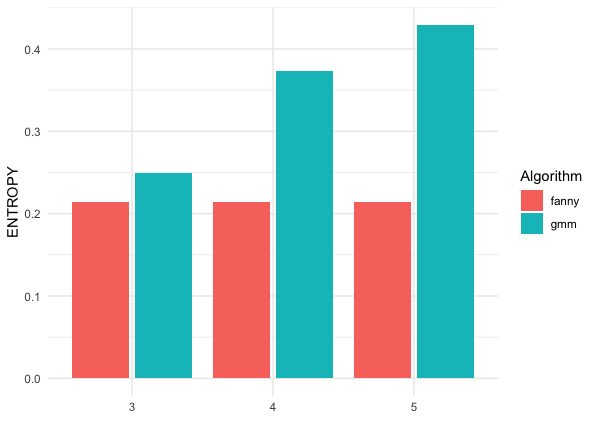
\includegraphics[width=6.5cm, height=4cm]{img/entropy} }}%
    \qquad
    \subfloat{{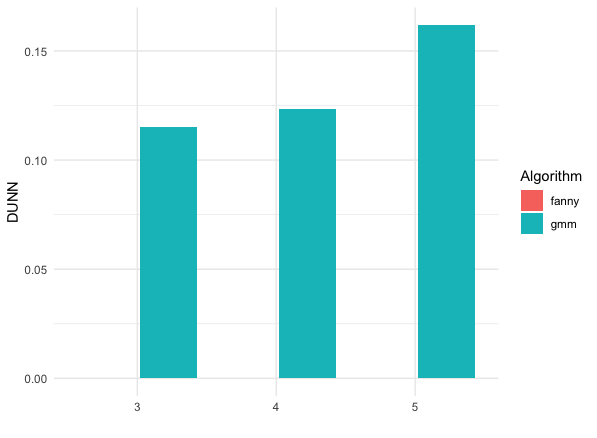
\includegraphics[width=6.5cm, height=4cm]{img/dunn} }}%
    \caption{Graphical representation of evaluation measures}%
    \label{fig:clustering}%
\end{figure}

\subsection*{Post-processing of data}

To conclude the definition of the methods of the package it is always necessary to have a functionality that allows us to sort, filter the information or export the data set. To do this we will detail the methods used:

\begin{itemize}
  \item \texttt{sort(clustering\_object,column\_name):} Sometimes it is necessary to determine what the maximum or minimum value of a column is and the easiest way to do this is by sorting the column. Here is an example of how to sort by column.
  \begin{Schunk}
\begin{Sinput}
> result <- Clustering::clustering(df = Clustering::basketball, min = 3, max=3,
\end{Sinput}
\begin{Sinput}
           algorithm = c('gmm'), metrics = c('entropy','dunn'))
 \end{Sinput}
\end{Schunk}
\begin{Schunk}
\begin{Sinput}
>  sort(result,F,'entropy')
\end{Sinput}
\begin{Soutput}
Result:
 Algorithm    Distance   Clusters   Dataset   entropy  dunn
   gmm    gmm_euclidean   3       dataframe  0.0000  0.1096
   gmm    gmm_manhattan   3       dataframe  0.0000  0.1151
   gmm    gmm_euclidean   3       dataframe  0.0032  0.1096
   gmm    gmm_manhattan   3       dataframe  0.0032  0.1151
   gmm    gmm_euclidean   3       dataframe  0.0064  0.1096
   gmm    gmm_manhattan   3       dataframe  0.0064  0.1151
   gmm    gmm_euclidean   3       dataframe  0.2120  0.1096
   gmm    gmm_manhattan   3       dataframe  0.2201  0.1151
   gmm    gmm_euclidean   3       dataframe  0.2374  0.1096
   gmm    gmm_manhattan   3       dataframe  0.2498  0.1151


\end{Soutput}
\end{Schunk}
  \item \texttt{"[.clustering":} There are times when we need to apply filters on a series of columns for a set of values. This process can be done using third party packages, but due to its great usefulness we have incorporated this functionality. To filter we must do it in the following way: clustering\_object [column\_1 operator value\_1 conditional\_1 .... column\_n operator value\_n]. Example of filtering:
  \begin{Schunk}
\begin{Sinput}
> result[entropy > 0.11 & dunn > 0.11 ]
\end{Sinput}
\begin{Soutput}
Result:
Algorithm   Distance      Clusters   Dataset    entropy dunn
   gmm     gmm_manhattan      3     dataframe   0.2498 0.1151
   gmm     gmm_manhattan      3     dataframe   0.2201 0.1151
\end{Soutput}
\end{Schunk}
  \item \texttt{Clustering::export\_file\_external():} exports the results of the clustering object to latex format This method is very useful when working with documents in latex format.
  \item \texttt{Clustering::export\_file\_internal():} this method is similar to the previous one, but only exports the internal metrics.
\end{itemize}


\section{Graphical User Interface of the \pkg{Clustering} package}

As mentioned throughout this paper, the \pkg{Clustering} package provides a GUI to work with clustering algorithms and to be able to evaluate and run the results more comfortable. The way to run the user interface is to execute the following instruction:

\begin{Schunk}
\begin{Sinput}
> Clustering::appClustering()
\end{Sinput}
\end{Schunk}

The execution will open our default browser with the interface. As it can be observed in the Figure ~\ref{fig:layoutApp}, we have a layout with header, side menu and main. In the header menu we can choose to see the numerical results or in graphical mode. In the left menu we can see the different parameters with which we can run our algorithm and finally in the central menu you can see the result of running the clustering algorithm.

\begin{figure}[htbp]
  \centering
   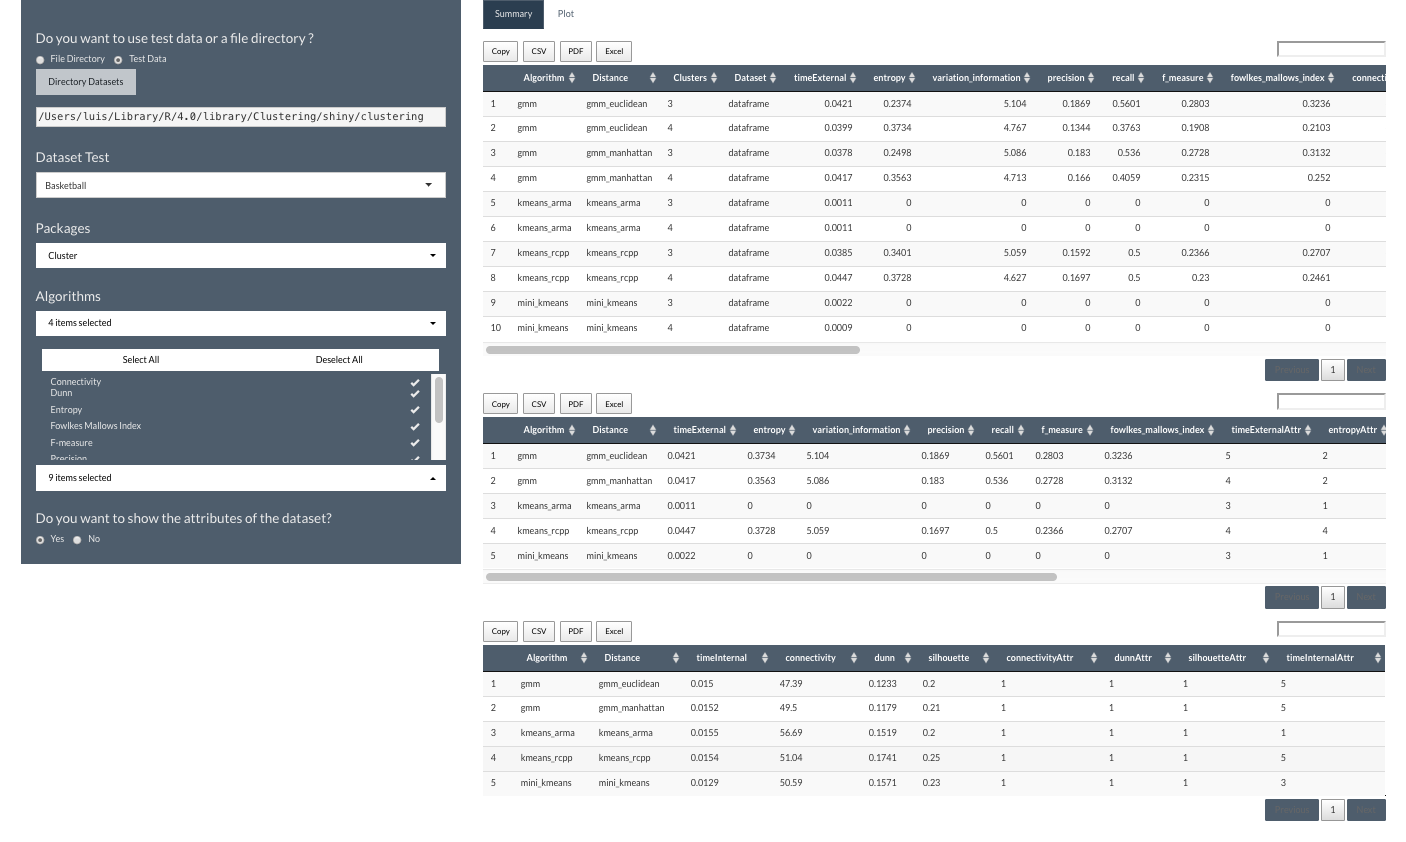
\includegraphics[width=14cm, height=9cm]{img/app}
    \caption{Clustering app user interface}
    \label{fig:layoutApp}%
\end{figure}

The operation of the application is very simple as can be seen in the Figure ~\ref{fig:layoutApp1} and we will proceed to explain it step by step.

\begin{figure}[htbp]
  \centering
   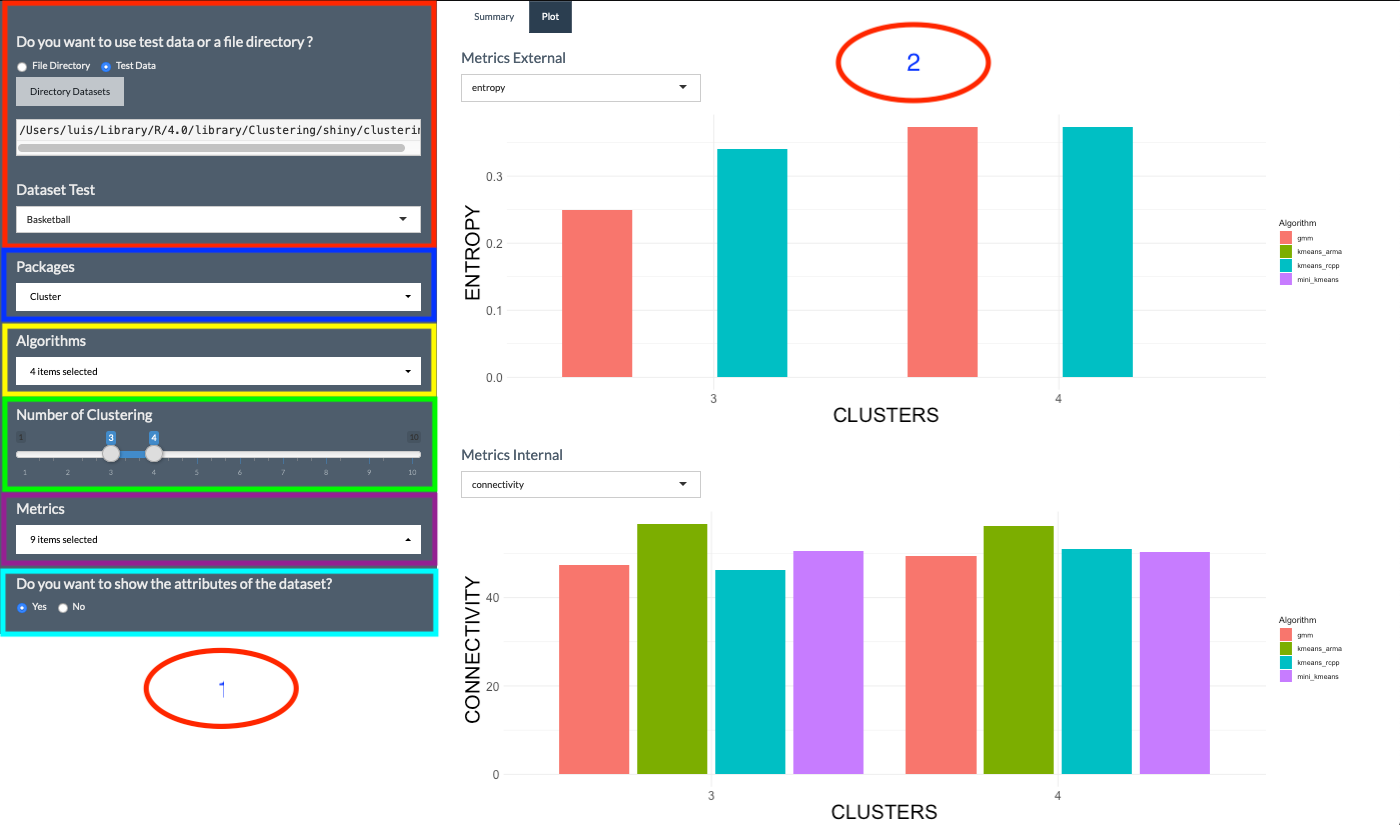
\includegraphics[width=14cm, height=9cm]{img/app1}
    \caption{Clustering app user interface}
    \label{fig:layoutApp1}%
\end{figure}

As you can see in the Figure ~\ref{fig:layoutApp1} we have two well differentiated parts:
\begin{enumerate}
  \item In this section we can find the different parameters used by the clustering function to filter the information.
  \begin{itemize}
  \item Marked in red, we can indicate if we want to work with test datasets or indicate a directory of dataset files to be processed.
  \item In blue we have the packages that implement the clustering algorithms mentioned throughout the paper. We can mark all the packages or individually. When a package is marked, all the algorithms implemented within the selected package are also marked.
  \item In yellow we have the algorithms implemented by the packages. If we mark an algorithm it will automatically mark its corresponding package in the package combo.
  \item In green we have the number of clusters. We can indicate ranges or select only one cluster by positioning the max and minimum on the same value.
  \item In violet we indicate the evaluation metrics used when validating the clusters.
  \item Finally we have a check through which instead of showing the metric values we can show the the dataset variable. In the image we have an example of execution with default variables.
\begin{figure}[htbp]
  \centering
   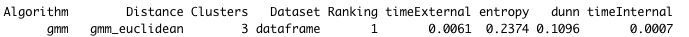
\includegraphics[width=14cm,height=0.5cm]{img/variable_false}
    \caption{Execution of the default \texttt{clustering} method}
    \label{fig:variable_false}%
\end{figure}
\\
In the Figure ~\ref{fig:variable_true} it is the execution of the same method with variable to true.
\begin{figure}[htbp]
  \centering
   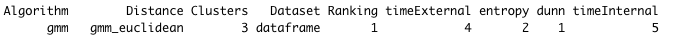
\includegraphics[width=14cm, height=0.5cm]{img/variable_true}
    \caption{Execution of the \texttt{clustering} method with variable to true}
    \label{fig:variable_true}%
\end{figure}
\\
Note: The variables in the data set can be translated into whole numbers. As we have worked with the basketball dataset throughout the paper, the dataset contains the following variables: \texttt{assists\_per\_minute, height, time\_played, age, points\_per\_minute}. These variables are translated into whole numbers from left to right, i.e. \texttt{assists\_per\_minute} corresponds to 1, \texttt{height} to 2 and so on. This is ideal, when instead of showing the numerical values of the metrics we need to see the variables of the set.
\end{itemize}
  \item In main layout we have the options to represent the data.
  \begin{itemize}

    \item To view the data in graphical mode as shown in the Figure ~\ref{fig:tab_graph}, we mark the Plot tab. In the figure we can see represented the internal and external evaluation metrics and depending on the type of evaluation we can filter individually by metrics to see the data represented graphically.

  \begin{figure}[htbp]
    \centering
     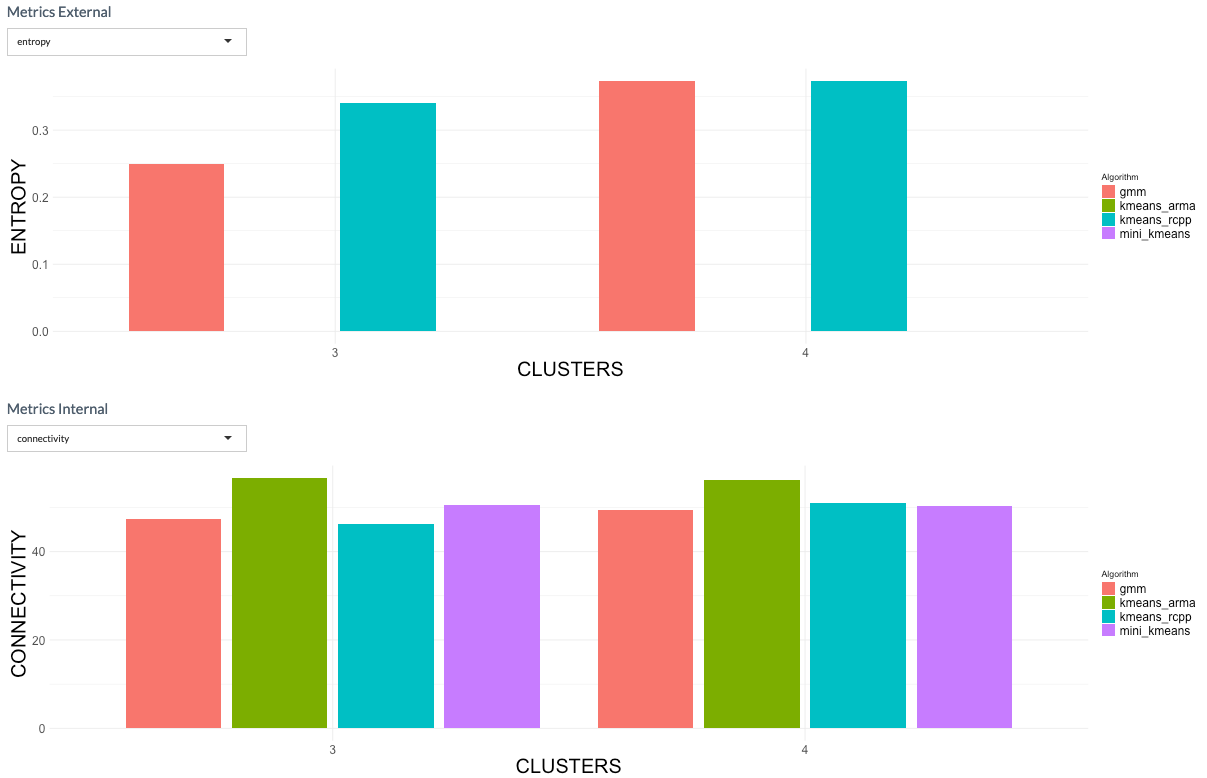
\includegraphics[width=14cm, height=8cm]{img/tab_graph}
      \caption{Tab with graphical representation of metrics}
      \label{fig:tab_graph}
  \end{figure}

    \item If we click on the summary tab as shown in the Figure ~\ref{fig:tab_summary}, we can see the data represented in tables. If you wish you can export the results in the following formats: csv,pdf and xls. We also have the option of copying the data.

  \begin{figure}[]
    \centering
     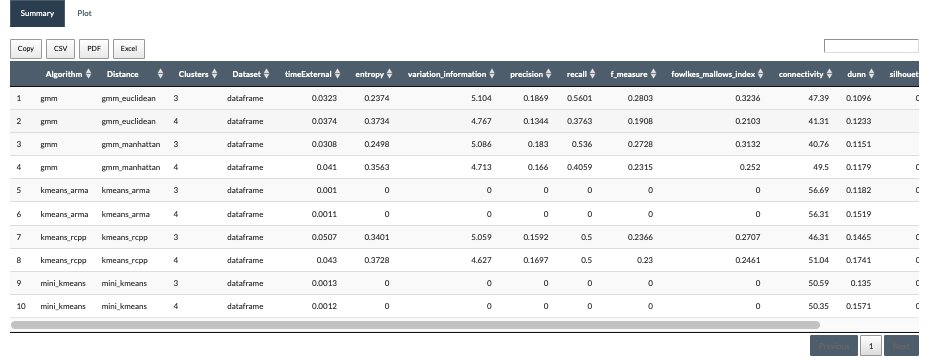
\includegraphics[width=14cm, height=3cm]{img/tab_summary}
      \caption{\pkg{Clustering} package execution summary tab}
      \label{fig:tab_summary}
  \end{figure}

  \end{itemize}

\end{enumerate}
\newpage
\section{Conclusion}

In this paper we have made an introduction to the \pkg{Clustering} package. The package has dependencies with other packages as seen throughout the paper. It allows the reading and loading of datasets in KEEL, CSV or ARFF format. We also offer the functionality of loading a \texttt{data.frame} in memory or using test datasets. As a complement the package has been enhanced with the inclusion of a graphical interface that allows the user to run the package in a simple way without the need to know the parameters. The development of the package will be continued with the inclusion of new algorithms, functionalities and improvement of the interface, therefore we encourage developers to contribute to the improvement of the package with the inclusion of new algorithms or functionalities or the inclusion of new proposals that complement the package.

\bibliography{RJreferences}

\address{Luis Alfonso Pérez Martos\\
  Computer Department\\
  University of Jaén\\
  Spain\\
  (ORCiD if desired)\\
  \email{lapm0001@gmail.com}}

\address{Ángel Miguel García Vico\\
  Computer Department\\
  University of Jaén\\
  Spain\\
  (ORCiD if desired)\\
  \email{agvico@ujaen.es}}

\address{Pedro González\\
  Computer Department\\
  University of Jaén\\
  Spain\\
  (ORCiD if desired)\\
  \email{pglez@ujaen.es}}

\address{Cristóbal J. Carmona\\
  Computer Department\\
  University of Jaén\\
  Spain\\
  (ORCiD if desired)\\
  \email{ccarmona@ujaen.es}}
